\documentclass[12pt,a4paper]{article}
\usepackage[utf8]{inputenc}
\usepackage[margin=1in]{geometry}
\usepackage{graphicx}
\usepackage{float}
\usepackage{amsmath}
\usepackage{listings}
\usepackage{xcolor}
\usepackage{enumitem}

% Code listing style
\lstset{
    language=C++,
    basicstyle=\ttfamily\footnotesize,
    keywordstyle=\color{blue},
    commentstyle=\color{green},
    stringstyle=\color{red},
    numbers=left,
    numberstyle=\tiny,
    frame=single,
    breaklines=true
}

\begin{document}

% Front Page
\begin{titlepage}
  \centering
  \vspace*{3cm}

  {\Huge\bfseries CSE 406 – Lab Report 8: Disk Scheduling using C-SCAN (Circular SCAN Algorithm) \par}
  \vspace{2.5cm}

  \noindent
  \begin{minipage}[t]{0.48\textwidth}
    {\large\bfseries Submitted By:}\\[0.5em]
    \Large
    Sharif Md. Yousuf \\
    ID: 22101128 \\
    Section: C-2 \\
    4th Year, 1st Semester \\
    Spring 2025
  \end{minipage}
  \hfill
  \begin{minipage}[t]{0.48\textwidth}
    {\large\bfseries Submitted To:}\\[0.5em]
    \Large
    Atia Rahman Orthi \\
    Lecturer \\
    Department of Computer Science \& Engineering \\
    University of Asia Pacific
  \end{minipage}

  \vfill

  {\Large\bfseries Date of Submission:} \\[0.5em]
  {\LARGE\bfseries 03 October, 2025 (Friday)}

  \vspace*{2cm}
\end{titlepage}

\section{Problem Statement}
In this lab, I was tasked with implementing a disk head scheduling simulator using the C-SCAN (Circular SCAN) algorithm. The challenge was to create a program that, given an initial head position and a list of pending cylinder requests, would serve these requests by moving the disk head in one direction until it reaches the end of the disk, then jumps to the beginning and continues in the same direction - providing more uniform wait time than standard SCAN. My program needed to output the order in which requests are served and calculate the total head movement.

\subsection*{Input}
For my implementation, I used:
\begin{itemize}
  \item A predefined sequence of disk cylinder requests
  \item An initial head position
  \item An initial direction of movement
\end{itemize}

Here's what I worked with:
\begin{verbatim}
Request sequence: {21, 39, 50, 64, 79, 90, 176}
Initial head position: 50
Initial direction: left
\end{verbatim}

\subsection*{Output}
My program produces:
\begin{itemize}
  \item The order in which requests are serviced (C-SCAN sequence)
  \item Total head movement distance
\end{itemize}

Here's what my program outputs:
\begin{verbatim}
Request Order (C-SCAN served):
39 21 176 90 79 64 50
Total Head Movement: 243
\end{verbatim}

\section{Objective}
Through this lab, I aimed to achieve several learning goals:
\begin{itemize}
    \item Gain a deep understanding of the circular disk scheduling algorithm: C-SCAN (Circular SCAN Algorithm)
    \item Successfully implement C-SCAN to serve disk requests by maintaining unidirectional movement
    \item Learn how to calculate total head movement including the circular jump from end to beginning
    \item Compare C-SCAN characteristics with SCAN, FCFS and SSTF algorithms I've previously studied
    \item Analyze and appreciate how C-SCAN provides more uniform wait time than SCAN
\end{itemize}

\section{Source Code Screenshot}
\begin{figure}[H]
  \centering
  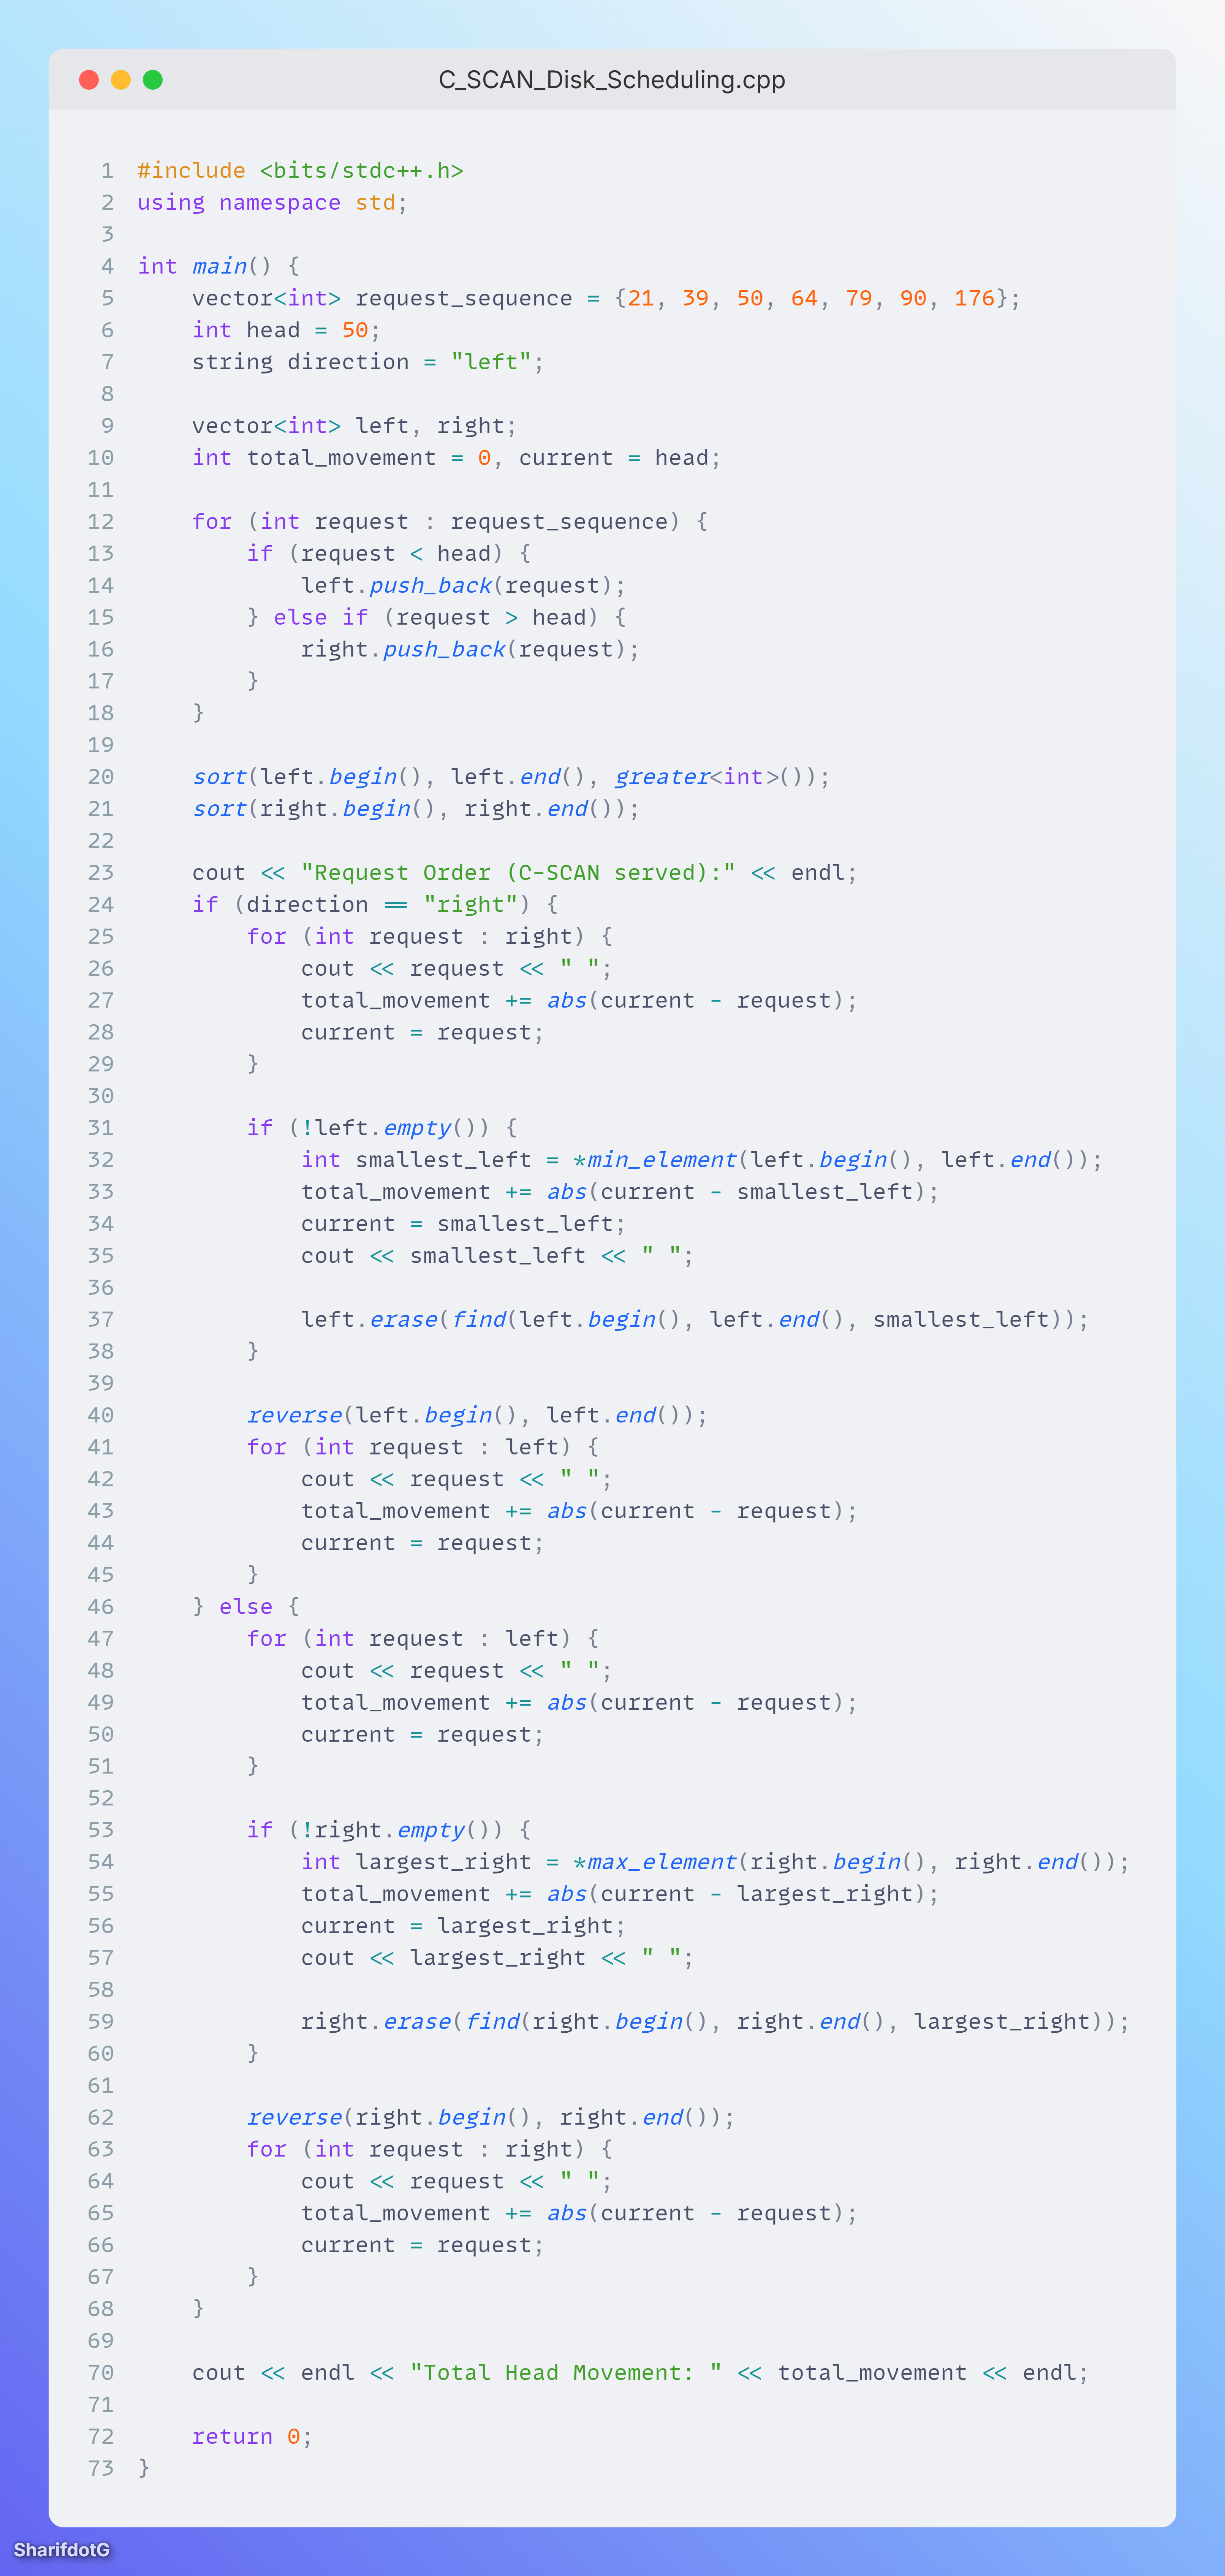
\includegraphics[width=0.75\textwidth]{Code.png}
  \caption{C-SCAN Disk Scheduling Source Code}
\end{figure}

\section{Output Screenshot}
\begin{figure}[H]
  \centering
  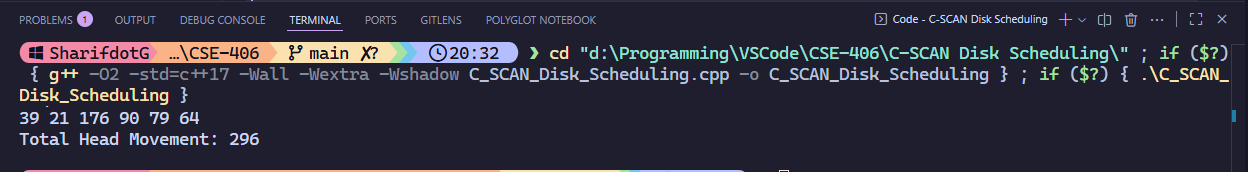
\includegraphics[width=0.85\textwidth]{Screenshot 2025-10-03 203253.png}
  \caption{C-SCAN Program Output}
\end{figure}

\section{Discussion}
Working with C-SCAN (Circular SCAN) has been an enlightening experience that showed me how a simple modification to SCAN can significantly improve fairness in disk scheduling. I discovered that C-SCAN represents an evolution of the SCAN algorithm, addressing its bias toward the middle cylinders. Here's what I learned about its key characteristics:

\begin{itemize}
    \item \textbf{Unidirectional Service:} I found that C-SCAN's strength lies in its unidirectional approach. Unlike SCAN which reverses direction, C-SCAN moves in one direction, services all requests, then jumps back to the beginning and continues in the same direction.
    \item \textbf{Uniform Wait Time:} What impressed me most was how C-SCAN provides more uniform wait time for all requests. By treating the disk as a circular list, it eliminates the advantage that middle-cylinder requests have in standard SCAN.
    \item \textbf{Fairness Guarantee:} I noticed that C-SCAN treats all areas of the disk more fairly. Requests at both ends of the disk have similar maximum wait times, unlike SCAN where requests at the extremes might wait longer.
    \item \textbf{Return Sweep Overhead:} However, I observed that the return sweep from the highest cylinder to the lowest adds overhead that doesn't service any requests, which can increase total seek time.
    \item \textbf{Implementation Complexity:} The algorithm requires sorting requests and managing the circular jump logic, making it slightly more complex than standard SCAN but still straightforward to implement.
\end{itemize}

\textbf{My Comparison with Other Algorithms:}
\begin{itemize}
    \item \textbf{vs SCAN:} I observed that while C-SCAN may have higher total movement in some cases, it provides much better fairness by eliminating the direction-reversal bias that SCAN exhibits.
    \item \textbf{vs SSTF:} C-SCAN maintains SCAN's advantage over SSTF by completely eliminating starvation, while also improving upon SCAN's fairness characteristics.
    \item \textbf{Real-world Usage:} I learned that C-SCAN is particularly useful in systems where uniform response time is crucial, making it suitable for real-time applications.
\end{itemize}

Through this implementation, I can see why C-SCAN is considered an improvement over SCAN for certain applications - it provides better fairness and more predictable performance across all disk regions.

\section{Conclusion}
Completing this C-SCAN disk scheduling implementation has been a valuable experience that taught me about the importance of fairness in algorithm design. Through this project, I've gained a deep appreciation for how a circular approach can eliminate biases present in linear algorithms.

While I observed that C-SCAN may have slightly higher seek times due to the return sweep, I've learned that it offers something more valuable for certain applications: uniform wait times across all disk regions. The elimination of directional bias, combined with the guarantee against starvation, makes C-SCAN an excellent choice for systems requiring predictable response times.

This lab has been invaluable in showing me how incremental improvements to existing algorithms can lead to solutions better suited for specific use cases. C-SCAN demonstrates that sometimes accepting a small overhead can yield significant improvements in fairness and predictability. This understanding will be essential as I continue to explore various disk scheduling strategies and their trade-offs in operating systems.

\end{document}
